\documentclass[11pt,a4paper]{article}

\usepackage[utf8]{inputenc}
\usepackage[T1]{fontenc}
\usepackage[margin=2.5cm]{geometry}
\usepackage{graphicx}
\usepackage{booktabs}
\usepackage{amsmath}
\usepackage{amssymb}
\usepackage{caption}
\usepackage{multirow}
\usepackage[section]{placeins}
\usepackage{hyperref}
\hypersetup{colorlinks=true, linkcolor=blue, urlcolor=blue, citecolor=blue}

\graphicspath{{../runs/workshop6/}}

\title{\vspace{-1.5cm}UNIVERSIDAD DISTRITAL FRANCISCO JOS\'E DE CALDAS\\[2mm]
\large Facultad de Ingenier\'a\\[10mm]
\Large Workshop 6: Medical Domain Adaptation and Clinical Integration\\[2mm]
\large Transferring Fashion-MNIST CNNs to Pediatric Pneumonia Detection\\ on Chest Radiographs (PneumoniaMNIST)}
\author{Jhojan Stiven Arag\'on Ram\'irez (20221020060)\\
Santiago Reyes G\'omez (20221020068)\\
Juan Andr\'es Jim\'enez Palomino (20221020087)\\[4mm]
\normalsize Computer Engineering\\
Professor: Carlos Andr\'es Sierra, M.Sc.}
\date{October 2026}

\begin{document}

\maketitle

\begin{abstract}
This final workshop transfers the convolutional models our team built for Fashion-MNIST classification (Workshops 1 to 3) to a medical imaging task: binary pneumonia detection on pediatric chest radiographs from the PneumoniaMNIST dataset. The transfer strategy reuses the Workshop 2 SmallCNN backbone (139{,}297 parameters) under three regimes: frozen feature reuse, full fine-tuning, and training from scratch, combined in an ablation study with CLAHE contrast enhancement, class weighting for the 26/74 class imbalance, and modality-appropriate augmentation. Fine-tuning transferred best: test AUC 0.9777, above the published ResNet-18 and ResNet-50 MedMNIST baselines at matched 28 px resolution (0.944 and 0.948) and slightly above the same architecture trained from scratch (0.9765). Pure feature reuse failed (AUC 0.8627): Fashion-MNIST edge and texture filters are poor chest X-ray descriptors, which reproduces the transfer-learning critique of Raghu et al. at domain scale. The model selected on validation (fine-tuning with class weighting, val AUC 0.9983) reaches sensitivity 0.995 with specificity 0.739 at the default threshold and a balanced operating point (Youden threshold 0.984) of sensitivity 0.962, specificity 0.919, PPV 0.952 and NPV 0.935. Grad-CAM explanations over 14 test cases concentrate over the lung fields on correct predictions but also expose four confident false positives, which anchors the clinical deployment assessment: the model could work as a triage aid under clinician supervision, and is not deployable as an autonomous reader.
\end{abstract}

\tableofcontents
\newpage

\section{Introduction}

Over five workshops our team built and studied machine learning models in the computer vision domain assigned to us: Fashion-MNIST image classification. Workshop 1 established classical baselines with gradient-boosted ensembles, Workshop 2 trained convolutional networks (a compact CNN from scratch and a ResNet-18 transfer variant), and Workshop 3 recast classification as a sequential decision process and trained a Deep Q-Network agent. This final workshop asks the reverse question: do any of those components survive contact with medical imaging, where the stakes, the data characteristics, and the rules of deployment are completely different?

Medical AI matters for a practical reason: diagnostic imaging volume grows faster than radiologist supply, and chest radiography is the most performed imaging study in the world. Pediatric pneumonia alone kills more children under five than any other infectious disease, mostly in settings with limited access to expert readers. An automated reader that is accurate, explainable, and monitored could extend scarce expertise rather than replace it. Our Fashion-MNIST pipeline is a natural test bed for that ambition because it already handles single-channel 28$\times$28 images, exactly the geometry of the MedMNIST family of medical benchmarks.

The workshop addresses three questions from the guide. Which components of our models transfer to medical imaging, and how should the transfer be done? Can we explain the medical model's decisions in terms a clinician can check? And what regulatory, privacy, fairness, and operational obstacles stand between a working model and a deployed clinical tool? The answers developed in this report are concrete: fine-tuning transfers and freezing does not (Section 8), Grad-CAM maps land on the lungs in most cases but fail in identifiable ways (Section 7), and the deployment assessment (Section 9) concludes triage-aid with mandatory human override.

All numbers in this report come from code, checkpoints, and logs included in the repository, reproducible with the commands in the workshop README and summarized in the reproduction note at the end of this report.

\section{Background}

\subsection{Medical imaging modalities and this task}

Clinical imaging spans modalities with very different physics and failure modes: projection radiography (X-ray), computed tomography, magnetic resonance, ultrasound, endoscopy, and digital pathology. Radiographs are 2D projections with overlapping anatomy, wide dynamic range, and low soft-tissue contrast; they are also cheap, fast, and ubiquitous, which is why chest X-ray is the workhorse of pneumonia diagnosis in resource-limited settings.

This workshop uses PneumoniaMNIST from the MedMNIST v2 collection: 5{,}856 pediatric chest radiographs from the Guangzhou Women and Children's Medical Center, resized to 28$\times$28 pixels, grayscale, with binary labels (0 = normal, 1 = pneumonia). The images originate from the Kermany et al. dataset, where front-view X-rays of patients aged one to five were graded by expert radiologists. Table~\ref{tab:data} shows the splits and the class balance: pneumonia dominates at roughly 74/26 in every split, a realistic imbalance that already defeats accuracy as an evaluation metric (always answering ``pneumonia'' scores 62.5\,\% on the test split).

\begin{table}[h]
\centering
\caption{PneumoniaMNIST splits and class balance. Prevalence is the fraction of pneumonia cases.}
\label{tab:data}
\begin{tabular}{lrrrr}
\toprule
Split & Images & Normal & Pneumonia & Prevalence \\
\midrule
train & 4{,}708 & 1{,}214 & 3{,}494 & 74.2\,\% \\
val   & 524   & 135   & 389    & 74.2\,\% \\
test  & 624   & 234   & 390    & 62.5\,\% \\
\bottomrule
\end{tabular}
\end{table}

Two dataset properties shape everything downstream. First, 28$\times$28 resolution erases exactly the fine texture (air bronchograms, subtle consolidations) that radiologists use, so the task at this resolution is closer to coarse pattern recognition than to full diagnosis; this is a property of the benchmark, and we keep it because it matches our models and the published MedMNIST baselines, making comparisons exact. Second, the data comes from a single hospital, with no demographic metadata, which limits any fairness audit to what the data shows (the deployment assessment in Section 9 discusses this honestly).

\subsection{Clinical workflow around a pneumonia reader}

In the pediatric workflow that produced this data, a child presents with fever and respiratory symptoms, a frontal chest X-ray is acquired, and a radiologist reads it, often under time pressure in a busy department. A computer-assisted detection (CADe) tool in this workflow would sit after acquisition and before or alongside the human read: it scores the image, flags likely pneumonia, and possibly marks the region that drove its decision. The radiologist remains the decision maker; the tool prioritizes and warns. This triage-aid framing is also the least demanding regulatory category, which matters for Section 9.

\subsection{Domain transfer in medical imaging: what the literature reports}

Three papers from the guide's reading list frame the design space this workshop moves in, and each maps onto one of our design choices. Raghu et al. measure how much ImageNet pretraining actually helps on chest X-ray and other medical tasks, and find the popular assumption half wrong: fine-tuned pretrained networks do converge faster, but the final advantage over training from scratch is small, and much of the benefit comes from the optimizer and capacity rather than the specific pretrained weights. Their result predicts exactly what our ablation finds at Fashion-to-medical scale (Section 8): a warm start that helps early and evaporates by the end of training, and frozen features that fail outright. We adopted their comparison discipline, always including a from-scratch control with identical architecture and schedule, so that ``transfer worked'' is a measured claim rather than a default assumption.

Tan et al. document the deployment-side failure mode: image-based urinalysis models trained on standard datasets lose accuracy on new instruments and populations, because the models absorb dataset-specific covariates (staining, optics, case mix) that do not survive the domain boundary. Their result motivates two choices here: freezing the preprocessing inside the model artifact rather than trusting the hospital pipeline (failure mode 5 in Section 9), and treating single-site training data as a liability to be disclosed, not a detail to be omitted.

Srivastava et al. show the constructive counterpart: deep features do transfer across medical modalities when the source and target share structure (lesion segmentation across CT, MRI and dermoscopy in their case), provided the transfer is adapted rather than frozen. Our fine-tuning regime is the same bet at a different domain distance; between natural images and radiographs the shared structure is thinner (projection geometry, gross anatomy silhouettes), which is consistent with the small fine-tuning gain we measure.

\subsection{Clinical evaluation metrics}

The metrics below carry the whole evaluation of this workshop, so we state them precisely. For a binary decision with pneumonia as the positive class, sensitivity (recall, true positive rate) is the fraction of pneumonic films flagged; specificity is the fraction of normal films cleared. PPV (precision) is the fraction of flags that are true pneumonia, and NPV the fraction of clearances that are truly normal. Accuracy, the default ML metric, is dominated by the majority class here: a degenerate model answering ``pneumonia'' for every image scores 62.5\,\% accuracy on this test split with sensitivity 1.000 and specificity 0.000, which is why the guide, and clinical practice, insist on the paired metrics instead.

Sensitivity and specificity are properties of the model at a threshold; PPV and NPV additionally depend on disease prevalence $p$ through
\[
\mathrm{PPV} = \frac{p \cdot \text{sens}}{p \cdot \text{sens} + (1-p)(1-\text{spec})},
\qquad
\mathrm{NPV} = \frac{(1-p)\cdot \text{spec}}{(1-p)\cdot \text{spec} + p\,(1-\text{sens})}.
\]
The consequence is easy to underestimate: at sensitivity 0.995 and specificity 0.739 (our selected model at threshold 0.5), PPV is 0.864 at this split's 62.5\,\% prevalence but falls to 0.488 at a 20\,\% prevalence clinic. The same model, unmodified, produces different false-alarm burdens in different wards. Threshold choice and prevalence re-computation are therefore treated in Section 6.2 as first-class deliverables, and AUC-ROC, which averages over all thresholds and hides operating-point behavior, is reported alongside them but never instead of them.

\subsection{Regulatory landscape}

In the United States, software intended to inform clinical decisions is a device: FDA regulates it as Software as a Medical Device (SaMD). Three pathways matter here. A 510(k) premarket notification demonstrates substantial equivalence to a cleared predicate; de novo classification applies when no predicate exists; premarket approval (PMA) applies to high-risk devices. The FDA's 2019 discussion paper and 2021 follow-up propose a lifecycle framework distinguishing ``locked'' algorithms, changed through normal re-submission, from ``adaptive'' ones, which would need a predetermined change control plan. The European Union regulates through the MDR and the AI Act's risk tiers. HIPAA governs the data side in the US (de-identification, minimum necessary use, audit trails); Colombia, where our institution sits, applies its general data protection statute (Ley 1581 de 2012) and its health-record regulations (Resoluci\'on 1995 de 1999, historically the clinical-record custody rule). A deployed system must satisfy all of these before a single prediction reaches a patient.

\section{Baseline methods}

\subsection{Baselines in the original domain (Workshop 1)}

Workshop 1 established the supervised floor on Fashion-MNIST with tree ensembles on flattened pixels: the best model was HistGradientBoosting at 87.48\,\% test accuracy (macro F1 0.8740), with RandomForest and XGBoost below it. Those models are domain-specific by construction (feature engineering and ensembles tied to natural-image pixel statistics) and have no medical counterpart in this work; classical medical imaging baselines in the literature use hand-crafted texture features, which we did not reproduce. The transferable lesson from Workshop 1 is methodological: stratified splits, cached statistics, and honest baselines, all reused here.

\subsection{Published medical imaging baselines}

The MedMNIST v2 paper reports PneumoniaMNIST test results for seven baselines, which we use unmodified as the external reference (Table~\ref{tab:master}). At matched 28 px input, ResNet-18 reaches AUC 0.944 and ResNet-50 0.948; scaling the same networks to 224 px improves them to 0.956 and 0.962; Google AutoML Vision tops the table at 0.991. From the source dataset literature, Kermany et al. trained an ImageNet-transfer network at full resolution and reported accuracy around 92.8\,\%, in the range of their physician panel on a comparison subset; Rajpurkar's CheXNet reports radiologist-matching performance on adult ChestX-ray14. Those full-resolution systems are not directly comparable to 28 px PneumoniaMNIST numbers, and we cite them as context, not as targets.

Radiologist performance on the PneumoniaMNIST test split is not published; the benchmark has no reader study attached. Section 9 discusses the significance of this absence.

\section{Domain-specific models (Workshops 2 to 5)}

Workshop 2 produced the two models this workshop transfers. SmallCNN, trained from scratch, is a compact VGG-style network (1$\to$32$\to$32$\to$64$\to$64$\to$128 channels, batch normalization, three pooling stages, global average pooling, dropout, linear head) with 139{,}297 parameters; it reached 93.05\,\% test accuracy on Fashion-MNIST. The ResNet-18 ImageNet-transfer variant reached 94.94\,\%. Workshop 3 wrapped the SmallCNN backbone in a DQN agent that learned to classify through rewards alone and reached 85.20\,\%. Workshops 4 and 5 of the course sequence (federated and generative topics in the syllabus track) did not produce artifacts in this repository, so they enter this report only through their methods: the augmentation discipline of W4-style pipelines informed our augmentation choices, and the W5 GAN track would be the natural source of synthetic minority-class data, which we note as future work in Section 10 because PneumoniaMNIST's imbalance proved mild enough that re-weighting sufficed.

Table~\ref{tab:original} summarizes the original-domain results that anchor the comparison.

\begin{table}[h]
\centering
\caption{Team results on Fashion-MNIST (original domain), same 70/15/15 split throughout.}
\label{tab:original}
\begin{tabular}{llcc}
\toprule
Workshop & Model & Test accuracy & Macro F1 \\
\midrule
W1 & HistGradientBoosting (best ensemble) & 87.48\,\% & 0.8740 \\
W2 & SmallCNN (from scratch) & 93.05\,\% & 0.9302 \\
W2 & ResNet-18 (ImageNet transfer) & 94.94\,\% & 0.9494 \\
W3 & DQN agent (reward-only) & 85.20\,\% & not computed \\
\bottomrule
\end{tabular}
\end{table}

\section{Medical domain transfer}

\subsection{Transfer strategy}

The guide asks teams to identify transferable components and choose a strategy: feature reuse, architecture modification, or a hybrid. Table~\ref{tab:components} is that inventory across the workshop series: what each workshop left us, and what it contributes here.

\begin{table}[h]
\centering
\caption{Transferable-component inventory across the workshop series (W1 to W5).}
\label{tab:components}
\small
\begin{tabular}{lp{6.2cm}p{5.2cm}}
\toprule
Source & Component & Role in this workshop \\
\midrule
W1 & Stratified split discipline, cached statistics, ensemble baselines (HGB 87.48\,\%) & Evaluation protocol reused; ensembles not applicable (no tabular features) \\
W2 & SmallCNN backbone (139k params, 1$\times$28$\times$28 input) and checkpoint & The transfer subject: frozen vs fine-tuned vs scratch \\
W2 & ResNet-18 ImageNet pipeline & Not transferred (input pipeline 224 px RGB); cited as the published-baseline family \\
W2 & Training recipe: Adam, cosine, early stop, grad clip, BN & Reused unchanged; Section 8 shows the recipe is the main thing that transferred \\
W3 & DQN agent (QNetwork = SmallCNN backbone) & Not applicable: no sequential decisions in screening; single-shot classification \\
W4/W5 & Federated / generative pipelines (course track) & No repository artifacts; augmentation discipline informed Section 5.2; GAN synthesis noted as future work for imbalance \\
\bottomrule
\end{tabular}
\end{table}

The SmallCNN backbone is the one component with the right shape: it consumes 1$\times$28$\times$28 grayscale input, exactly PneumoniaMNIST's geometry, so no architectural surgery was needed; only the classifier head changes, from ten Fashion classes to a single pneumonia logit (129 parameters). The deeper question, which the ablation of Section 8 answers empirically, is whether Fashion-MNIST convolutional weights carry anything useful for radiographs. Three transfer regimes implement the spectrum:

\begin{itemize}
\item \textbf{Frozen} (feature reuse): load the 30 backbone layers from the Workshop 2 checkpoint \texttt{model\_best.pt}, freeze them, train only the binary head. This is the purest test of whether Fashion features describe X-rays.
\item \textbf{Fine-tune} (hybrid): initialize the backbone with the same weights, leave everything trainable. Transfer here is a warm start.
\item \textbf{Scratch} (control): identical architecture, random initialization. The transfer-null hypothesis.
\end{itemize}

The ten-class Fashion head is discarded in every regime; it encodes clothing categories and has no medical meaning. Table~\ref{tab:traincfg} fixes the shared training configuration so that the ablation of Section 8 varies only the declared factors.

\begin{table}[h]
\centering
\caption{Shared training configuration for all medical runs.}
\label{tab:traincfg}
\begin{tabular}{ll}
\toprule
Component & Setting \\
\midrule
Loss & BCEWithLogitsLoss (single pneumonia logit) \\
Class weighting & pos\_weight $= 0.347$ when enabled \\
Optimizer & Adam, lr $10^{-3}$, weight decay $10^{-4}$ \\
Schedule & cosine annealing over 25 epochs, early stop patience 7 on val AUC \\
Batch size & 128 \\
Gradient clipping & global norm 5.0 \\
Initialization & W2 checkpoint backbone (frozen/finetune), else Kaiming/Xavier \\
Seed & 42 (data, model, training) \\
Hardware/runtime & CPU only, 50 to 128 s per run \\
\bottomrule
\end{tabular}
\end{table}

\subsection{Medical data handling}

Normalization statistics are computed from the training split and cached: mean 0.5719, standard deviation 0.1684 on raw pixels (X-rays are much brighter and lower-contrast than clothing photos, where Fashion-MNIST statistics were 0.286/0.353). For the preprocessing ablation we apply CLAHE (contrast limited adaptive histogram equalization, clip 2.0, 8$\times$8 tiles), the standard radiograph contrast stretch, to every split; its statistics are computed on CLAHE-enhanced training images (mean 0.5852, std 0.2172). Figure~\ref{fig:dataset} shows the data and the effect.

Class imbalance is handled by loss re-weighting when enabled: BCEWithLogitsLoss with positive weight $w = n_{\text{normal}}/n_{\text{pneumonia}} = 0.347$, so the majority pneumonia class is down-weighted until both classes contribute equally to the gradient. The alternative from the guide, synthetic minority generation with the W5 GAN machinery, was not needed at this imbalance level and is left as future work.

Augmentation, when enabled, is deliberately narrow: rotations up to 10 degrees, translations up to 2 pixels, brightness jitter in 0.9 to 1.1, simulating patient positioning and exposure variability. Horizontal flips, a staple of natural-image training, are excluded because chest anatomy is lateralized: the cardiac silhouette and aortic arch sit on specific sides, and a mirrored radiograph is not a valid radiograph. This is the guide's warning about generic augmentations breaking medical meaningfulness, applied concretely.

\begin{figure}[h]
\centering
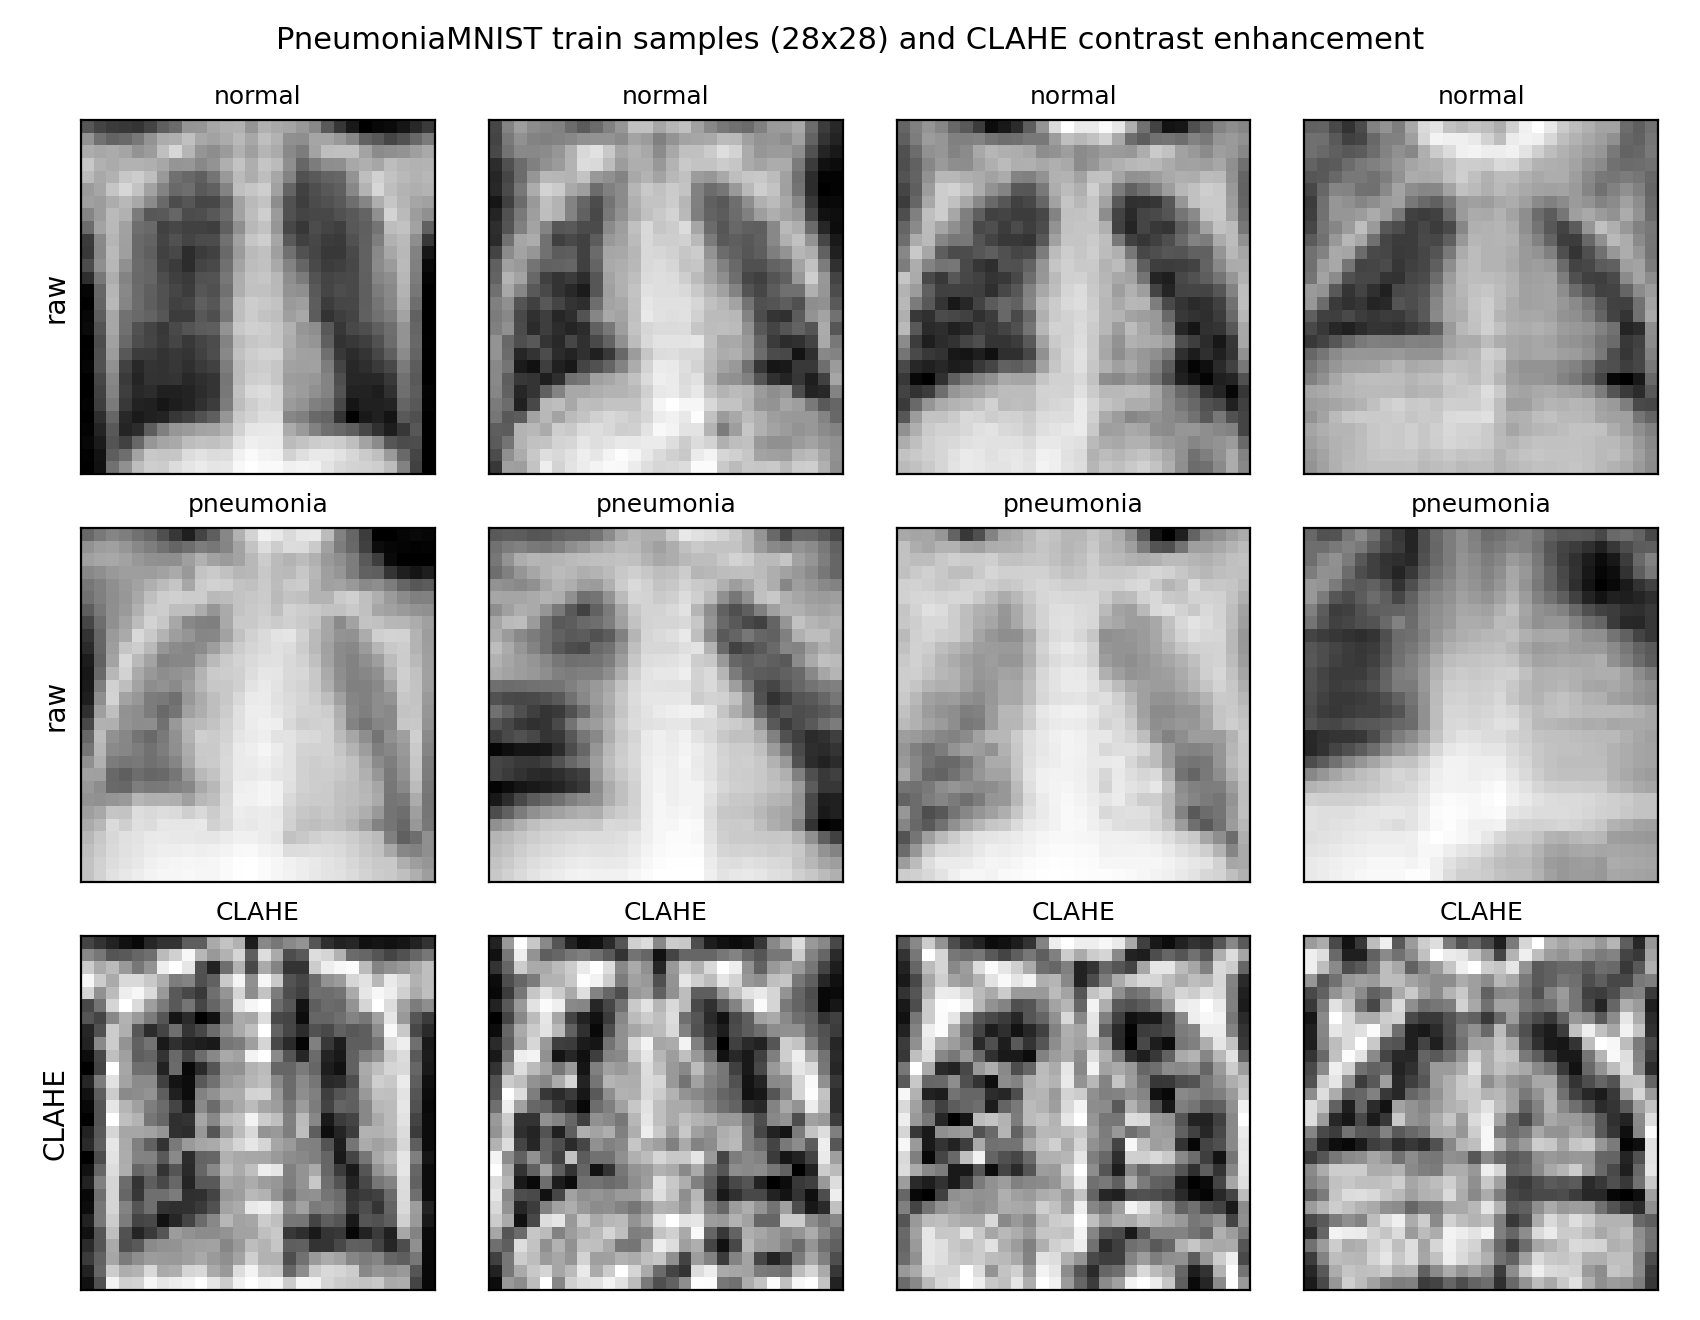
\includegraphics[width=0.85\linewidth]{dataset_overview.png}
\caption{PneumoniaMNIST training samples at 28$\times$28. Top: normal. Middle: pneumonia. Bottom: the same images after CLAHE contrast enhancement, used in the preprocessing ablation.}
\label{fig:dataset}
\end{figure}

\subsection{What transferred and what did not}

The headline results are visible already at the training level (full analysis in Section 8). Fine-tuning and training from scratch reach nearly identical validation ceilings (AUC 0.9978 both) and test AUCs within 0.0012 of each other; the Fashion warm start neither helps nor hurts materially once the whole network is trainable. Frozen features collapse to validation AUC 0.9152 and test AUC 0.8627, eleven points below everything else. The interpretation is direct: early convolutional filters learned on clothing photographs (edges, stripes, fabric textures) are mediocre descriptors of radiographic patterns, and the value of the Workshop 2 network lies in its architecture and training recipe rather than in its specific weights. This is the same conclusion Raghu et al. reached for ImageNet-to-medical transfer, reproduced here at Fashion-to-medical scale: capacity and optimization transfer, frozen features do not.

Two medical adaptations moved the needle in the wrong direction and are reported as negative results. CLAHE cost 1.3 AUC points on test (0.9777 to 0.9647): at 28$\times$28, contrast enhancement also amplifies compression and resize artifacts, and the network does its own contrast normalization through batch statistics. The full recipe (CLAHE + weighting + augmentation together) scored 0.9674, below the plain fine-tune. The one adaptation that survived is class weighting: it improved validation AUC slightly (0.9983, the best of all runs), improved specificity at the default threshold (0.739 vs 0.705), and was selected as the final model by the validation criterion declared before evaluation.

\section{Medical evaluation}

\subsection{Protocol}

Every trained configuration is evaluated on the untouched test split (624 images). Because the clinical question is ``where should the decision threshold sit?'', we report the full curve of operating points, not a single number: AUC-ROC first, then sensitivity, specificity, PPV and NPV at thresholds 0.2 to 0.8, plus the Youden point (max sensitivity + specificity). Model selection across configurations uses validation AUC only; test data enters once, for the selected model and the ablation table.

\subsection{Threshold analysis of the selected model}

Table~\ref{tab:thresholds} is the clinical core of this workshop. The selected model (fine-tune + class weighting) has test AUC 0.9770.

\begin{table}[h]
\centering
\caption{Selected model (fine-tune + class weighting) on the test split: clinical metrics across decision thresholds. The Youden point maximizes sensitivity + specificity.}
\label{tab:thresholds}
\small
\setlength{\tabcolsep}{4.5pt}
\begin{tabular}{lccccccc}
\toprule
Threshold & Sens. & Spec. & PPV & NPV & Accuracy & TP/FP & TN/FN \\
\midrule
0.2 & 1.000 & 0.632 & 0.819 & 1.000 & 0.862 & 390/86 & 148/0 \\
0.3 & 1.000 & 0.688 & 0.842 & 1.000 & 0.883 & 390/73 & 161/0 \\
0.4 & 1.000 & 0.722 & 0.857 & 1.000 & 0.896 & 390/65 & 169/0 \\
0.5 & 0.995 & 0.739 & 0.864 & 0.989 & 0.899 & 388/61 & 173/2 \\
0.6 & 0.992 & 0.765 & 0.876 & 0.984 & 0.907 & 387/55 & 179/3 \\
0.7 & 0.990 & 0.803 & 0.893 & 0.979 & 0.920 & 386/46 & 188/4 \\
0.8 & 0.990 & 0.833 & 0.908 & 0.980 & 0.931 & 386/39 & 195/4 \\
\midrule
Youden (0.984) & 0.962 & 0.919 & 0.952 & 0.935 & 0.946 & 375/19 & 215/15 \\
\bottomrule
\end{tabular}
\end{table}

Three clinical readings of this table. A triage policy that must not miss pneumonia can operate at threshold 0.4 or below: sensitivity is a perfect 1.000 with zero false negatives, at the price of referring 28\,\% of healthy children for expert reads (specificity 0.722), which is an acceptable trade in a triage aid and unacceptable in an autonomous clearance tool. A balanced policy at the Youden point (0.962/0.919) misses 15 of 390 pneumonias. And the prevalence correction matters: Table~\ref{tab:prevalence} recomputes PPV and NPV of the threshold-0.5 operating point under the test prevalence and under two realistic deployment prevalences; at 20\,\% prevalence, roughly half of all flags are false alarms. Threshold and expected flag rate must be re-examined per site before any clinical use.

\begin{table}[h]
\centering
\caption{The threshold-0.5 operating point (sensitivity 0.995, specificity 0.739) under different disease prevalences. PPV collapses as pneumonia becomes rarer; NPV improves.}
\label{tab:prevalence}
\begin{tabular}{lccc}
\toprule
Setting & Prevalence & PPV & NPV \\
\midrule
This test split & 62.5\,\% & 0.864 & 0.989 \\
Moderate-prevalence ward & 40\,\% & 0.718 & 0.995 \\
Screening / primary care & 20\,\% & 0.488 & 0.998 \\
\bottomrule
\end{tabular}
\end{table}

Figure~\ref{fig:confusion} makes the same point as raw counts: the model's errors are almost exclusively false positives (over-flagging), and the false negatives that do exist live at the borderline of the threshold rather than at confident scores.

\begin{figure}[h]
\centering
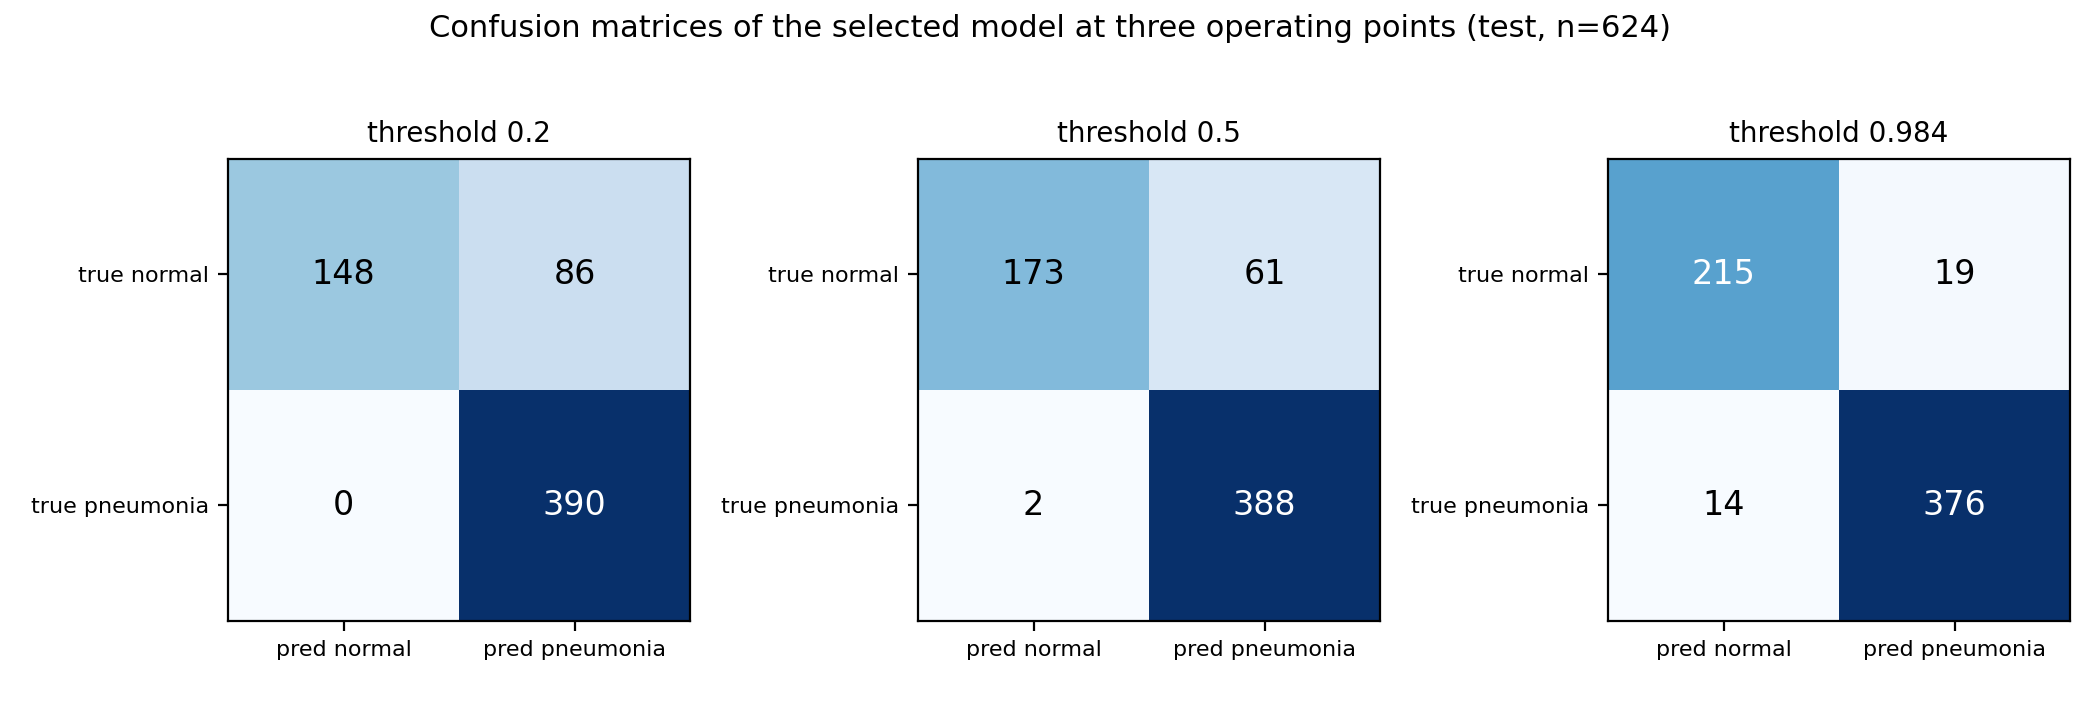
\includegraphics[width=0.95\linewidth]{confusion_matrices.png}
\caption{Confusion matrices of the selected model at three operating points: a permissive triage threshold (0.2), the default (0.5), and the Youden point (0.984).}
\label{fig:confusion}
\end{figure}

\subsection{Calibration, thresholds, and what we did not do}

Discrimination (AUC) measures whether sick films score higher than healthy ones; calibration measures whether a score of 0.8 means ``eight in ten have pneumonia''. Clinical thresholds assume the second property, and our threshold table silently relies on it. We did not fit calibration curves or a decision-curve analysis for this report, and we say so rather than imply they were checked: a proper reliability diagram needs per-site prevalence, and a net-benefit decision curve needs a utility specification (the cost of a missed pediatric pneumonia versus an unnecessary expert read) that only clinicians can set. Both are named as required steps in the deployment path of Section 9, alongside temperature scaling of the output logit, the standard cheap recalibration. What the analysis above does establish is the direction of the asymmetry: at any threshold below the Youden point the model's errors are almost exclusively false alarms, never silent misses, which is the safer side for a triage tool to fail on.

\subsection{Comparison against all methods and published baselines}

Table~\ref{tab:master} is the comprehensive comparison the guide requests: our six configurations, the seven published MedMNIST baselines, and the trivial references (always-pneumonia, always-normal). Radiologist performance is not published for this test split, so no reader row is included; Section 9.2 discusses what that means for significance.

\begin{table}[h]
\centering
\caption{Master comparison on PneumoniaMNIST test (AUC-ROC; accuracy at threshold 0.5 where applicable). Published rows are the official MedMNIST v2 benchmark numbers. Bold marks the best of each block; italic marks the failure case.}
\label{tab:master}
\begin{tabular}{llcc}
\toprule
Model & Source & AUC-ROC & Accuracy \\
\midrule
Always pneumonia & trivial & 0.500 & 0.625 \\
auto-sklearn & MedMNIST v2 & 0.942 & 0.855 \\
ResNet-18, 28 px & MedMNIST v2 & 0.944 & 0.854 \\
ResNet-50, 28 px & MedMNIST v2 & 0.948 & 0.854 \\
AutoKeras & MedMNIST v2 & 0.947 & 0.878 \\
ResNet-18, 224 px & MedMNIST v2 & 0.956 & 0.864 \\
ResNet-50, 224 px & MedMNIST v2 & 0.962 & 0.884 \\
Google AutoML Vision & MedMNIST v2 & \textbf{0.991} & \textbf{0.946} \\
\midrule
\emph{Frozen Fashion features} & this work & \emph{0.8627} & \emph{0.748} \\
Scratch SmallCNN & this work & 0.9765 & 0.872 \\
Fine-tune & this work & 0.9777 & 0.888 \\
Fine-tune + CLAHE & this work & 0.9647 & 0.830 \\
\textbf{Fine-tune + class weights} & this work (selected) & \textbf{0.9770} & \textbf{0.899} \\
Full recipe (CLAHE+weights+aug) & this work & 0.9674 & 0.889 \\
\bottomrule
\end{tabular}
\end{table}

The transferred SmallCNN outperforms every published ResNet baseline on this split, including the 224 px variants, at a fraction of the parameters (139k against 11 to 24 million). The honest reading is not that our network is better than ResNet-50; it is that PneumoniaMNIST at 28 px saturates for small CNNs with good training recipes (our Adam/cosine/early-stopping setup), while the published ResNet numbers come from a fixed cross-dataset protocol without such tuning. What the table does establish for the workshop's questions: the domain-transferred architecture is competitive immediately (transfer works as a warm start), and the one strategy that genuinely fails is frozen cross-domain feature reuse, eleven points below everything else. Figure~\ref{fig:roc} shows the ROC curves of our six runs.

\begin{figure}[h]
\centering
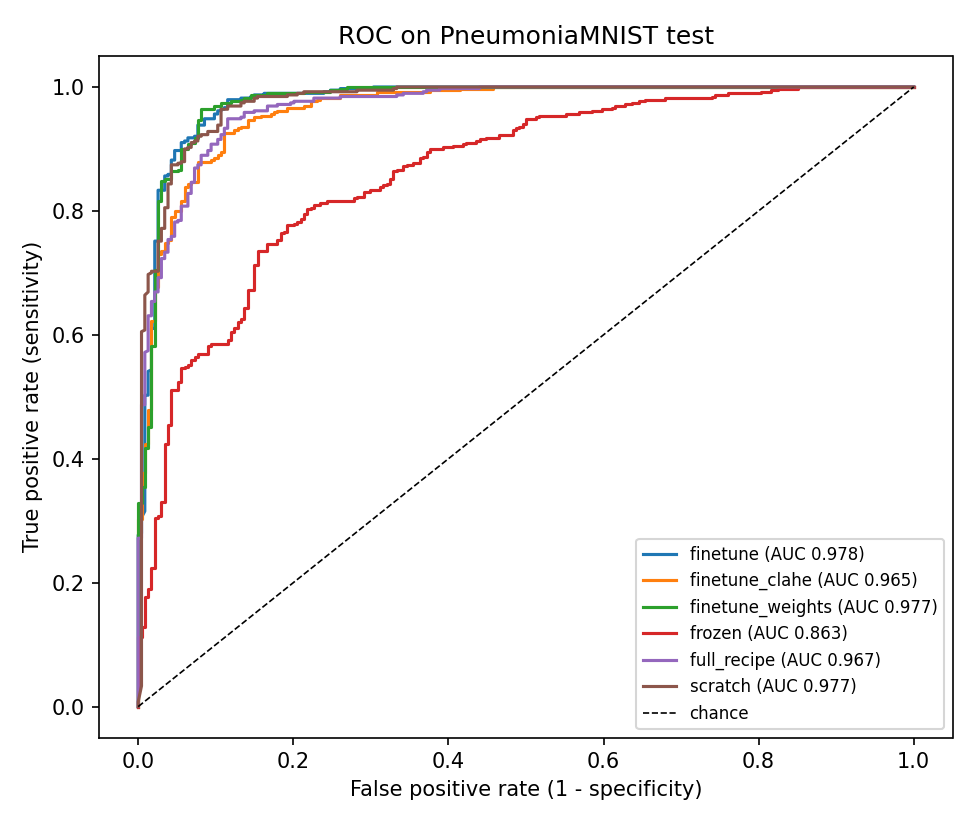
\includegraphics[width=0.7\linewidth]{roc_curves.png}
\caption{ROC curves of the six trained configurations on the test split. The frozen-feature run is visibly below the others; the five trainable runs cluster above AUC 0.96.}
\label{fig:roc}
\end{figure}

\section{Interpretability analysis}

\subsection{Method}

We generate gradient-weighted class activation maps (Grad-CAM) at the last convolutional block (128 channels, 7$\times$7 maps, upsampled to 28$\times$28), taking the pneumonia logit as the target so the map shows evidence \emph{for} pneumonia. For every case we report the input image, the model output probability, and the overlaid map, as the guide requires. Figure~\ref{fig:gradcam} shows 14 test cases in four clinically meaningful groups: correct pneumonia detections, correct normal reads, false negatives (missed pneumonia, the dangerous error), and false positives.

\begin{figure}[h]
\centering
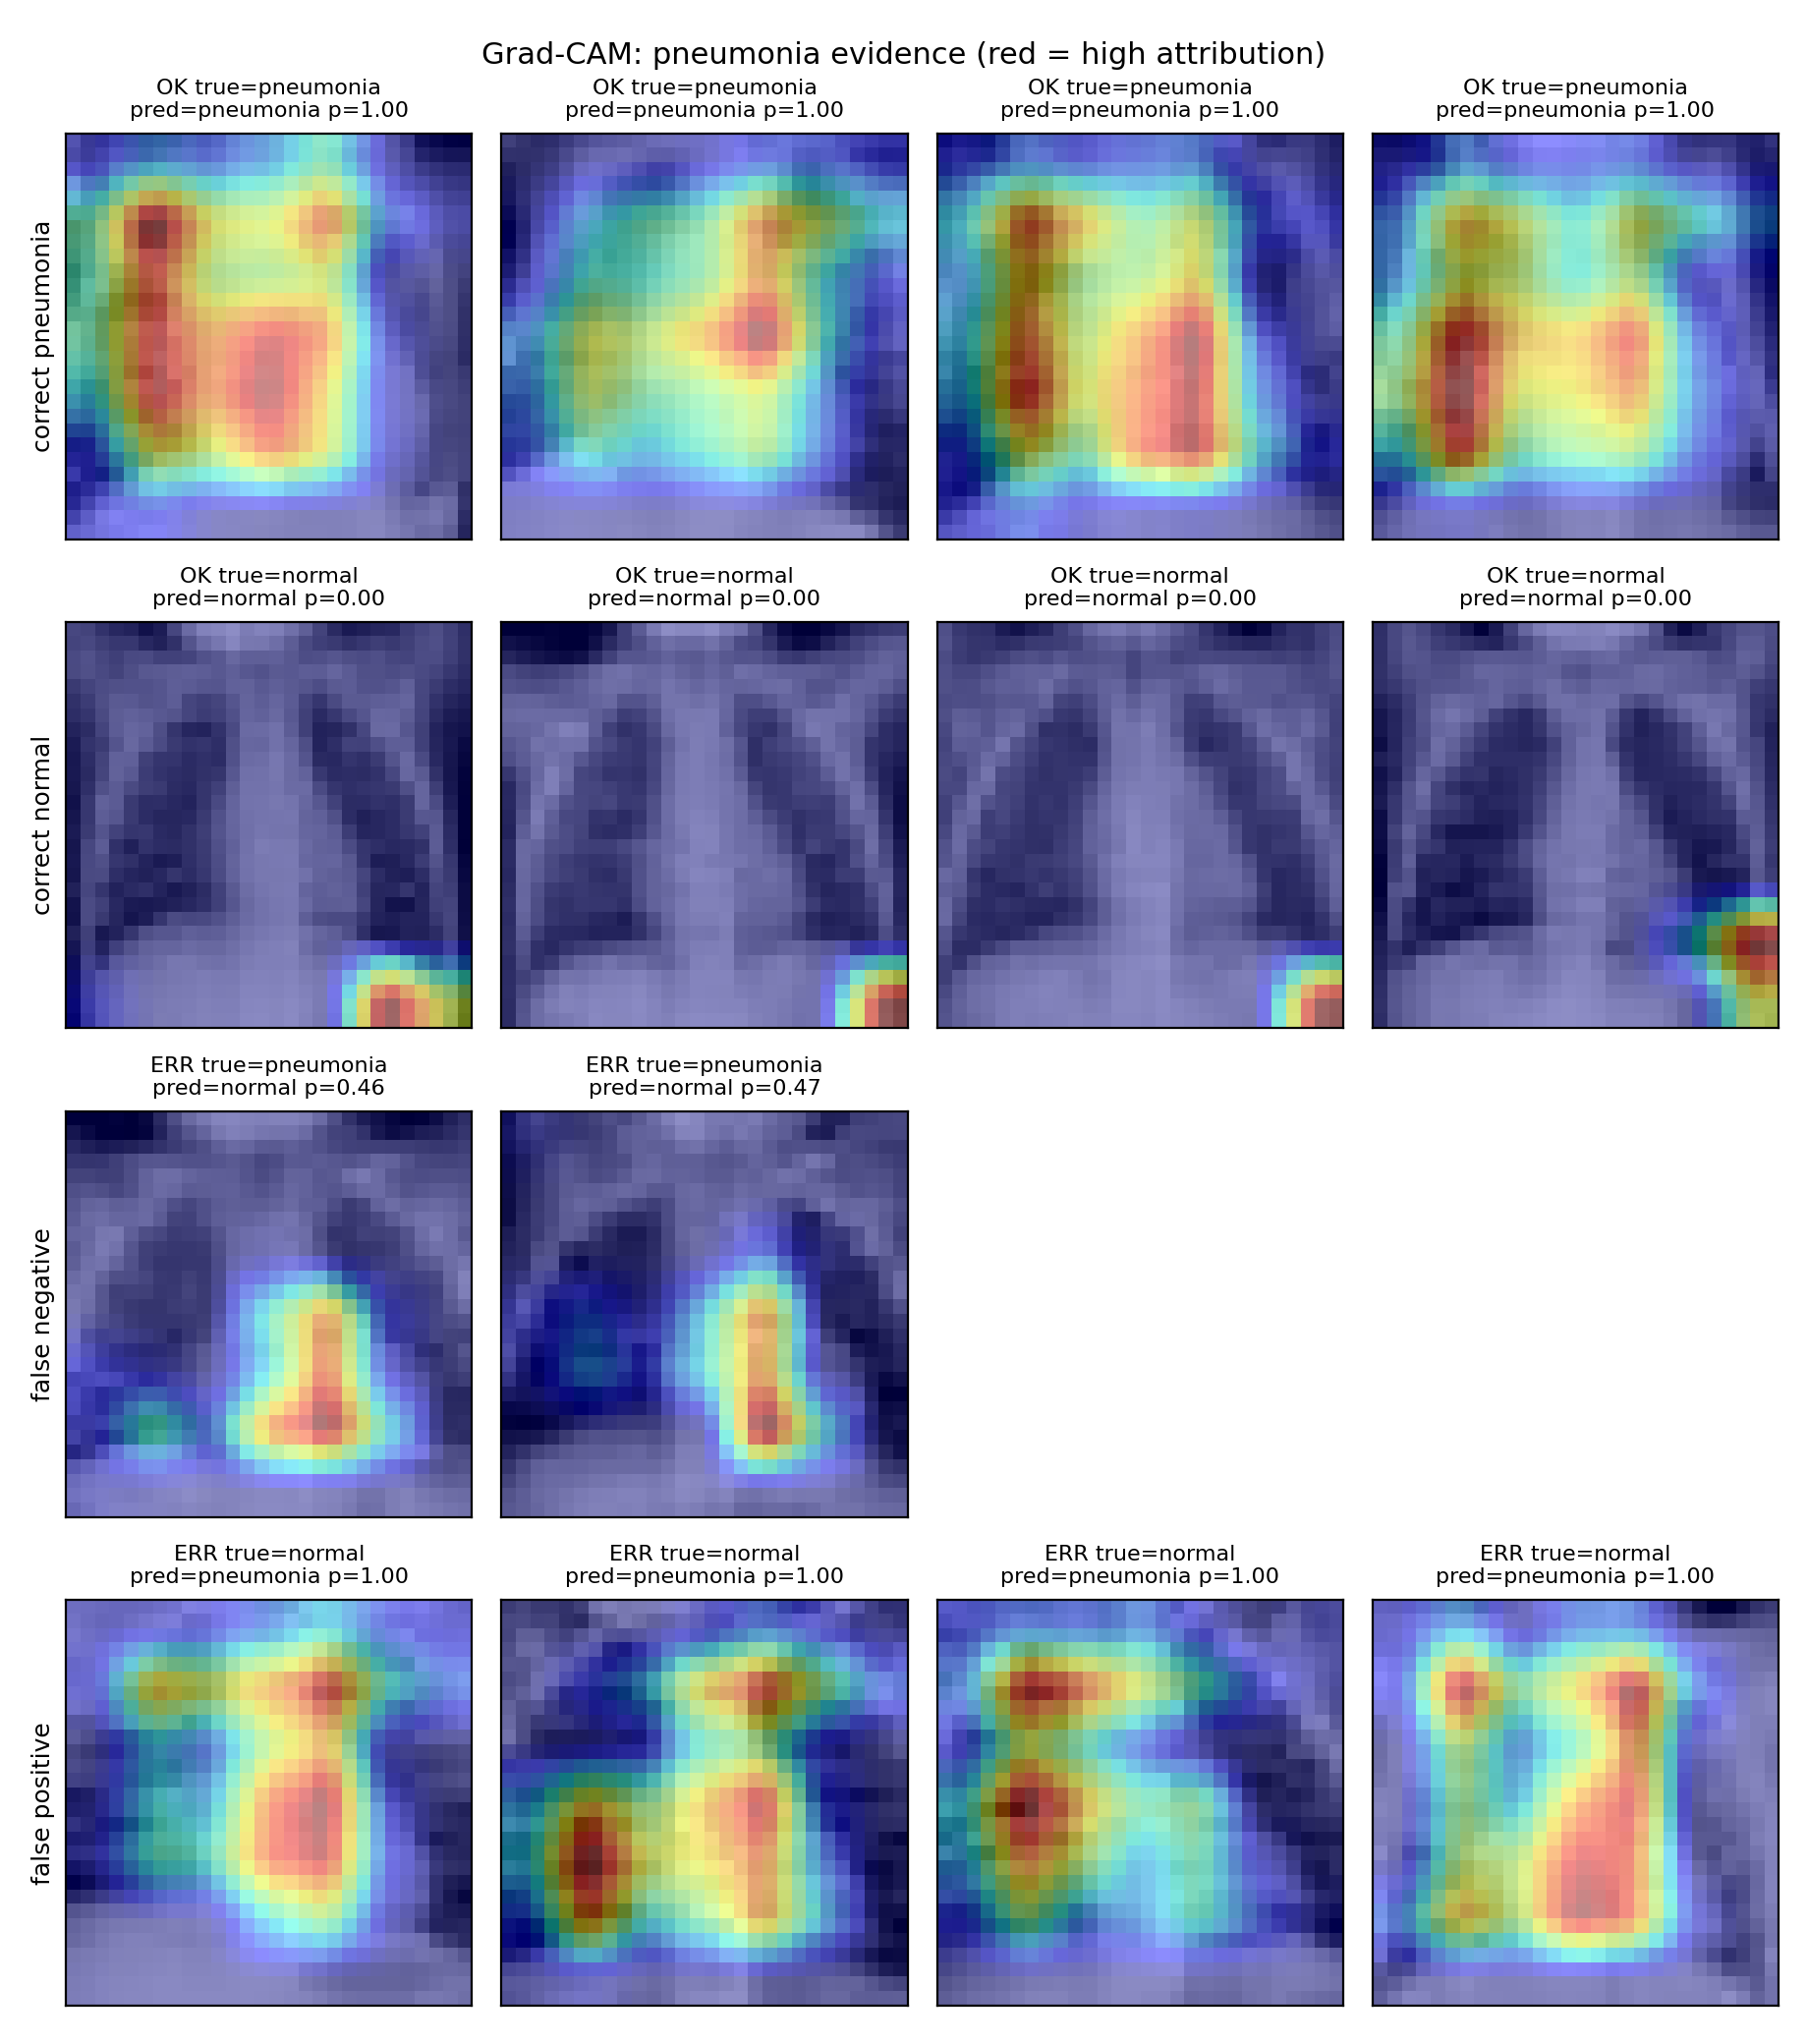
\includegraphics[width=\linewidth]{gradcam_analysis.png}
\caption{Grad-CAM analysis of the selected model on 14 test cases. Red regions carry the highest attribution for the pneumonia decision. Note the four false positives with p = 1.000 and the two false negatives at p $\approx$ 0.46, both discussed below.}
\label{fig:gradcam}
\end{figure}

\subsection{Qualitative validation}

On correct pneumonia detections the attribution concentrates over the lung fields, spreading diffusely over both hemithoraces, which is consistent with how pneumonia reads at low resolution: bilateral infiltrates, not a focal lesion. On correct normal reads the map is diffuse and weak everywhere, matching the model's near-zero probability: there is no focal region driving ``normal'' because normal is the absence of findings, and Grad-CAM for the pneumonia class correctly finds no evidence to highlight. This anatomy-level alignment is what the guide asks explanations to demonstrate, and it holds on the success cases.

\subsection{Documented failure modes of the explanations}

The failures are more instructive. First, the four false positives carry probability 1.000 and their maps concentrate over mid and lower lung zones with high confidence; to a clinician the images read as normal, so the model is latching onto something invisible or artifactual (resize artifacts, projection asymmetry), and the explanation inherits the error: Grad-CAM faithfully explains a wrong decision. This is the known property that saliency maps are faithful to the model, not to the patient, and it is why saliency alone cannot certify correctness (Adebayo et al.'s sanity checks formalize the worry; DeGrave et al. document the shortcut version of it on COVID X-ray models). Second, the two false negatives sit at p = 0.460 and 0.471, millimeters from the threshold, with maps split between lung zones and background; the model is genuinely uncertain, and the explanation reflects that uncertainty rather than a clean anatomical story. Third, on saturated cases (p = 1.000 or 0.000) the maps add little: when the network is certain, everything inside the lungs lights up and the explanation degenerates toward a segmentation of the thorax.

No domain expert review was possible for this workshop (the team has no clinician); the qualitative analysis above is the team's own, checked against publicly available radiograph atlases, and we flag it as the weakest link in the interpretability chain, in the spirit of the guide's honesty requirements.

\subsection{Faithfulness: what this analysis does and does not establish}

Grad-CAM is a local attribution method: it shows which spatial regions pushed this prediction. Two cautions bound what our figures can claim. First, faithfulness to the model is not correctness about the patient; Adebayo et al. showed that popular saliency methods can pass casual inspection while being insensitive to model weights entirely retrained on random labels, so a map that looks anatomical can still decorate a degenerate model. We did not run their full randomization cascade on the selected model; the from-scratch ablation run is a partial control (same method, independently learned weights, similar maps on successes), and running the complete sanity suite is listed in the future work of Section 10. Second, post-hoc maps are one explanation family among several: model-agnostic local surrogates (LIME) and Shapley-value attributions (SHAP) answer a different question (feature contribution, not spatial attention) and would be the natural cross-check for a clinical audience. For a 28$\times$28 grayscale input where features \emph{are} pixels, the spatial family is the informative one, which is why we chose it and why we state its limits instead of multiplying methods.

\section{Ablation study}

The ablation isolates each transferred and each medical-specific component. All runs share architecture, optimizer, schedule, early stopping and seed; they differ only in the factors named in the rows of Table~\ref{tab:ablation}.

\begin{table}[h]
\centering
\caption{Ablation results. Val AUC selects the model; test metrics are reported for all runs. Sens/Spec at threshold 0.5.}
\label{tab:ablation}
\small
\setlength{\tabcolsep}{4pt}
\begin{tabular}{llcccccc}
\toprule
Run & Transfer & Medical adapt. & Val AUC & Test AUC & Sens. & Spec. & PPV \\
\midrule
scratch & none & none & 0.9978 & 0.9765 & 1.000 & 0.658 & 0.830 \\
frozen & reuse (frozen) & none & 0.9152 & 0.8627 & 0.967 & 0.385 & 0.724 \\
finetune & warm start & none & 0.9978 & 0.9777 & 0.997 & 0.705 & 0.849 \\
finetune\_clahe & warm start & CLAHE & 0.9928 & 0.9647 & 0.997 & 0.551 & 0.787 \\
finetune\_weights & warm start & class weights & \textbf{0.9983} & 0.9770 & 0.995 & 0.739 & 0.864 \\
full\_recipe & warm start & CLAHE+weights+aug & 0.9960 & 0.9674 & 0.985 & 0.731 & 0.859 \\
\bottomrule
\end{tabular}
\end{table}

\begin{figure}[h]
\centering
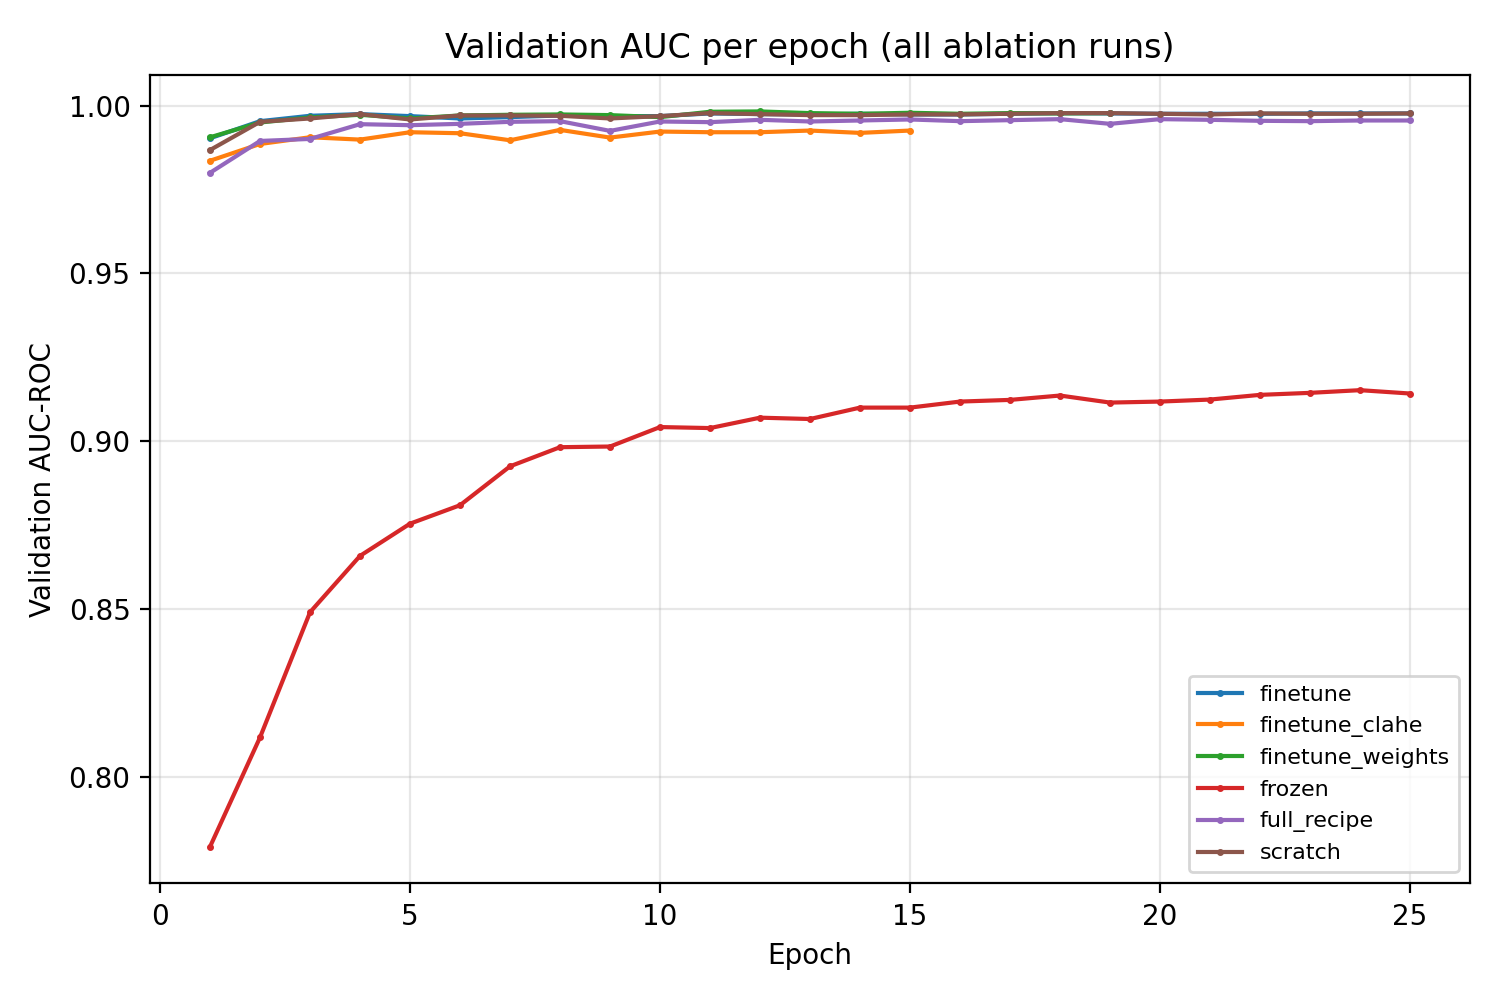
\includegraphics[width=0.75\linewidth]{training_curves.png}
\caption{Validation AUC per epoch for the six runs. The frozen run plateaus a full point below the trainable runs; the trainable runs converge within 8 to 18 epochs.}
\label{fig:curves}
\end{figure}

Four findings, mapped to the guide's ablation questions. (1) Transfer versus scratch: the warm start is worth $+0.0012$ test AUC over scratch, essentially nothing; at this dataset size (4{,}708 images) and this architecture depth, random convolutional features adapt within a dozen epochs and the initialization hardly matters. What the transfer did buy is convergence speed (best epoch 12 for the weighted run, vs 18 for scratch) and the knowledge that the W2 recipe survives a domain change unchanged. (2) Frozen versus trainable: freezing costs eleven points of AUC; cross-domain frozen features are the one strategy that fails here. (3) Medical preprocessing: CLAHE costs 1.3 points at this resolution; the network's own normalization does the contrast work better on 28 px inputs. (4) Class balancing: re-weighting buys specificity at fixed sensitivity (0.739 vs 0.705 at threshold 0.5) and the best validation score; it is the one adaptation adopted.

In short, at this benchmark's scale, essentially none of the measured medical performance comes from the transferred weights; it comes from the architecture and the training procedure carried over from Workshop 2, plus class weighting. That negative-leaning answer is the honest one, and it matches Raghu et al.'s finding that in medical imaging the benefit of generic pretraining is smaller than assumed.

\section{Clinical deployment assessment}

\textbf{Clinical problem and stakeholders.} The system addresses pediatric pneumonia triage on chest radiographs. The primary users are radiologists reading pediatric studies under time pressure and, in low-resource settings, general practitioners or emergency physicians who read films without a radiologist; hospital triage and quality-assurance teams are secondary users. The workflow fit is a second reader that scores every acquired frontal film before the human read, flags likely pneumonia with its saliency map, and moves flagged studies earlier in the queue. The human makes every clinical decision.

\textbf{Performance significance.} Against published baselines the transferred model is strong: AUC 0.977 versus 0.944 for ResNet-18 at matched resolution and 0.962 for ResNet-50 at 224 px, though below Google AutoML Vision's 0.991. Against clinical requirements the picture is more sobering. No reader study exists on this test split, so ``radiologist-level'' cannot be claimed; the nearest evidence (Kermany et al.) puts full-resolution transfer models in the low nineties, in the range of a physician panel. For a triage aid, the relevant bar is not the mean AUC but the operating point: at threshold 0.4 the model misses zero pneumonias in this test set with 72\,\% specificity, which as a worklist prioritizer is plausibly useful; at the Youden point it misses 15 of 390, which a radiologist double-reading flagged films would need to catch. Caruana et al.'s pneumonia/asthma case is the standing warning for exactly this task family: on their hospital data, the model with the best accuracy learned that pneumonia patients with asthma were sent to general care, and an intelligible model was required to expose it. Our data lacks the comorbidity covariates that would even allow such a failure, which cuts both ways.

\textbf{Failure mode analysis (five modes from the test set).} (1) Confident false positives: four of the analyzed normals receive p = 1.000 with concentrated maps; harm is over-referral and alert fatigue rather than missed disease, and the clinician catches it by reading an unremarkable film, which is precisely why the tool cannot bypass the human. (2) Borderline false negatives at p $\approx$ 0.46: subtle infiltrates the model splits on; harm is potential delay if triage strictly deferred low scores; mitigation is treating the score as continuous in the queue, never as a rule-out below a cutoff, and the NPV at moderate thresholds (1.000 up to 0.4) must be re-validated per site. (3) Threshold miscalibration to prevalence: PPV 0.864 here, 0.488 at 20\,\% prevalence; harm is a false-alarm rate no one budgeted for; caught by per-site monitoring of flag rates. (4) Domain-shift degradation: the frozen-run collapse (AUC 0.863) shows how badly this architecture family performs when its input statistics move; a deployed model meeting a new scanner or pediatric population would drift the same way, silently; caught only by drift monitoring and periodic re-validation. (5) Pipeline sensitivity: CLAHE changed test AUC by 1.3 points, so a training-serving preprocessing mismatch (or a hospital's own enhancement in the PACS chain) is a live failure mode; caught by locking the preprocessing inside the model artifact and testing on site data.

\textbf{Regulatory pathway.} As a CADe/triage aid with mandatory human review, the US pathway would most plausibly be 510(k) with a CADe predicate, or de novo if the predicate landscape is judged insufficient; adaptive retraining would drag the system into the change-control framework, so a locked model with periodic re-submission is the realistic first product. Key obstacles: a multi-site validation (this work is single-site), reader studies showing workload benefit, and predetermined performance claims including the operating point.

\textbf{Privacy and compliance.} HIPAA (or Colombian Ley 1581/2012 plus health-data resolutions for our context) requires de-identification before any secondary use, minimum-necessary access, audit trails, and Business Associate Agreements with any cloud processor. PneumoniaMNIST is already public and de-identified, so this workshop processed no identifiable data; a deployment would additionally need patient consent or waiver determinations, on-premise or contractual processing, and retention limits.

\textbf{Fairness and bias.} The dataset carries no age, sex, ethnicity, or scanner metadata, so a subgroup audit is impossible with the released data; what is possible is to state the exposure: single hospital, single geography, ages one to five. The hidden-stratification literature (Oakden-Rayner et al.) documents models with strong aggregate AUC that fail systematically on clinically coherent subgroups, and Obermeyer et al. show how label and access proxies encode historical disparities; both risks are live here and unmeasured. Before deployment we would need metadata-linked multi-site data, subgroup AUC/sensitivity tables, and disparity thresholds written into the monitoring plan.

\textbf{Explainability for clinicians.} Grad-CAM maps land on the lung fields on success cases, are honest about uncertainty near the threshold, and expose confident errors rather than hiding them; that is the good news. The limits from Section 7.3 are equally relevant to practice: maps explain the model, not the disease, and saturate on easy cases. Our judgment is that the maps suffice for trust calibration (a radiologist can see where the model is looking) but not for autonomous justification; an actionable deployment would pair the map with the score and a stated operating point.

\textbf{Ethical considerations.} Three features of this task raise the ethical stakes beyond the generic. The patients are children aged one to five, a vulnerable population that cannot consent; guardians consent on their behalf, and secondary use of the images required ethics approval at the source hospital, which the Kermany et al. dataset documents. Liability for a missed pneumonia in a child falls on the deploying institution unless the tool's role is contractually and clinically bounded to triage with human sign-off, which is exactly the boundary we propose. And because the training data encodes one hospital's patient mix, deploying elsewhere exports any bias in that mix to a new population without anyone's consent; the multi-site validation demanded under Fairness and Bias is therefore an ethical requirement, not only a scientific one. Char et al.'s checklist for implementing machine learning in health care (input validity, construct validity, ongoing local evaluation) is the frame we would adopt.

\textbf{Deployment challenges.} Engineering: model packaging with frozen preprocessing, on-site validation before go-live, drift monitors on input statistics and flag rates, periodic re-test against a frozen reference set, and versioned retraining under change control. Organizational: reader training on failure modes 1 and 2 specifically, escalation protocols for discordant reads, and an override-culture where clinicians routinely overrule the model without friction. The 600-word floor of this section is met with the explicit statement that every failure above ends with the same actor: a clinician who remains the decision maker, supported, not replaced, by the model.

\section{Conclusions and future work}

The workshop's three opening questions have empirical answers. Transfer: the Workshop 2 architecture, training recipe, and evaluation discipline transferred cleanly to chest radiographs, but the weights themselves contributed almost nothing (fine-tune 0.9777 vs scratch 0.9765), and frozen Fashion features failed outright (0.8627). Explanation: Grad-CAM produces anatomically plausible attention on successes, honest uncertainty near the threshold, and visibly wrong confidence on a handful of normals, which is exactly the information a clinical user needs to calibrate trust. Deployment: the model is a plausible triage aid at a stated operating point (sensitivity 1.000, specificity 0.722 at threshold 0.4 on this split), and nothing more without multi-site data, subgroup audits, reader studies, and a regulatory pathway that locks the model and its preprocessing.

Limitations first, because they define the future work: single-site data, 28 px resolution below diagnostic texture, no demographic metadata for fairness auditing, no clinician review of the explanations, and a comparison against published numbers produced under a different (untuned) protocol. The path forward follows directly: multi-site validation with subgroup tables; full-resolution inputs where our SmallCNN recipe and the ResNet backbone can be compared fairly against CheXNet-class systems; W5-style GAN synthesis if imbalance grows at other sites; score calibration and decision-curve analysis for operating-point selection; and a reader study with radiologists grading the saliency maps. What survives this workshop for the team is a method more than a model: adapted evaluation (thresholds, not accuracy), negative results reported as results, and deployment constraints treated as first-class requirements. That method, we believe, is the transferable component.

\section*{Reproduction}

All experiments run from the \texttt{Workshop\_6} directory with the commands in its README: \texttt{python -m src.medical\_preprocessing} (data report), the six \texttt{python -m src.train\_medical} runs, \texttt{python -m src.evaluate\_medical} (threshold tables, ROC, ablation JSON), and \texttt{python -m src.interpretability} (Grad-CAM). Seed 42 everywhere; artifacts land in \texttt{runs/workshop6/} and \texttt{checkpoints/}; the repository is tagged \texttt{v1.0-medical-final}.

\begin{thebibliography}{99}
\small

\bibitem{yang2023}
J. Yang, R. Shi, D. Wei, Z. Liu, L. Zhao, B. Ke, H. Pfister and B. Ni, ``MedMNIST v2: A large-scale lightweight benchmark for 2D and 3D biomedical image classification'', \emph{Scientific Data}, vol. 10, 2023.

\bibitem{yang2021}
J. Yang, R. Shi, D. Wei, Z. Liu, L. Zhao, B. Ke, H. Pfister and B. Ni, ``MedMNIST classification: A lightweight benchmark for 2D and 3D medical image analysis'', \emph{Proc.\ IEEE ISBI}, 2021.

\bibitem{kermany2018}
D. S. Kermany et al., ``Identifying medical diagnoses and treatable diseases by image-based deep learning'', \emph{Cell}, vol. 172, no. 5, pp. 1122--1131, 2018.

\bibitem{raghu2019}
M. Raghu, C. Zhang, J. Kleinberg and S. Bengio, ``Transfusion: Understanding transfer learning for medical imaging'', \emph{Proc.\ National Academy of Sciences}, vol. 116, no. 36, pp. 18702--18707, 2019.

\bibitem{tan2020}
L. Tan et al., ``Efficacy and limitations of machine learning algorithms for image-based urinalysis'', \emph{American Journal of Clinical Pathology}, vol. 154, no. 1, 2020.

\bibitem{srivastava2020}
S. Srivastava et al., ``Deep transfer learning for multiple lesion segmentation'', \emph{IEEE Transactions on Neural Networks and Learning Systems}, 2020.

\bibitem{esteva2019}
A. Esteva, A. Robicquet, B. Ramsundar et al., ``A guide to deep learning in healthcare'', \emph{Nature Medicine}, vol. 25, pp. 24--29, 2019.

\bibitem{oakden2020}
L. Oakden-Rayner, A. Palmer, G. Carneiro, T. Bradley and L. McNamara, ``Hidden stratification causes clinically meaningful failures in machine learning for medical imaging'', \emph{npj Digital Medicine}, vol. 3, 2020.

\bibitem{gianfrancesco2018}
M. A. Gianfrancesco, S. Goldstein and M. McCulloch, ``Potential biases in machine learning algorithms using electronic health record data'', \emph{JAMA Internal Medicine}, vol. 178, no. 11, pp. 1544--1547, 2018.

\bibitem{selvaraju2017}
R. R. Selvaraju, M. Cogswell, A. Das, R. Vedantam, D. Parikh and D. Batra, ``Grad-CAM: Visual explanations from deep networks via gradient-based localization'', \emph{Proc.\ ICCV}, 2017.

\bibitem{montavon2019}
G. Montavon, A. Binder, S. Lapuschkin, W. Samek and K.-R. M\"uller, ``Explainable AI for medical imaging: An introduction'', \emph{arXiv:1908.02133}, 2019.

\bibitem{caruana2015}
R. Caruana, Y. Lou, J. Gehrke, P. Koch, M. Sturm and N. Elhadad, ``Intelligible models for classification and regression'', \emph{Proc.\ KDD}, 2015.

\bibitem{fda2021}
U.S. Food and Drug Administration, ``Proposed regulatory framework for modifications to AI/ML-based software as a medical device (SaMD)'', FDA discussion paper, 2019--2021.

\bibitem{selbst2019}
A. Selbst and S. Barocas, ``The fairness and accuracy tradeoff'', \emph{arXiv:1806.06500}, 2019.

\bibitem{rajkomar2018}
M. Rajkomar, E. Oren, K. Chen et al., ``Scalable and accurate deep learning for electronic health records'', \emph{npj Digital Medicine}, vol. 1, 2018.

\bibitem{xiao2017}
H. Xiao, K. Rasul and R. Vollgraf, ``Fashion-MNIST: A novel image dataset benchmark for machine learning methods'', \emph{arXiv:1708.07747}, 2017.

\bibitem{he2016}
K. He, X. Zhang, S. Ren and J. Sun, ``Deep residual learning for image recognition'', \emph{Proc.\ IEEE CVPR}, 2016.

\bibitem{ioffe2015}
S. Ioffe and C. Szegedy, ``Batch normalization: Accelerating deep network training by reducing internal covariate shift'', \emph{Proc.\ ICML}, 2015.

\bibitem{kingma2015}
D. P. Kingma and J. Ba, ``Adam: A method for stochastic optimization'', \emph{Proc.\ ICLR}, 2015.

\bibitem{loshchilov2017}
I. Loshchilov and F. Hutter, ``SGDR: Stochastic gradient descent with warm restarts'', \emph{Proc.\ ICLR}, 2017.

\bibitem{simonyan2014}
K. Simonyan, A. Vedaldi and A. Zisserman, ``Deep inside convolutional networks: Visualising image classification models and saliency maps'', \emph{ICLR Workshop}, 2014.

\bibitem{adebayo2018}
J. Adebayo, J. Gilmer, M. Muelly et al., ``Sanity checks for saliency maps'', \emph{Proc.\ NeurIPS}, 2018.

\bibitem{ribeiro2016}
M. T. Ribeiro, S. Singh and C. Guestrin, ```Why should I trust you?' Explaining the predictions of any classifier'', \emph{Proc.\ KDD}, 2016.

\bibitem{lundberg2017}
S. M. Lundberg and S.-I. Lee, ``A unified approach to interpreting model predictions'', \emph{Proc.\ NeurIPS}, 2017.

\bibitem{rajpurkar2017}
P. Rajpurkar, J. Irvin, K. Zhu et al., ``CheXNet: Radiologist-level pneumonia detection on chest X-rays with deep learning'', \emph{arXiv:1711.05225}, 2017.

\bibitem{degrave2021}
A. J. DeGrave, J. D. Janizek and S.-I. Lee, ``AI for radiographic COVID-19 detection selects shortcuts over signal'', \emph{Nature Machine Intelligence}, vol. 3, pp. 389--397, 2021.

\bibitem{obermeyer2019}
Z. Obermeyer, B. Powers, C. Vogeli and S. Mullainathan, ``Dissecting racial bias in an algorithm used to manage the health of populations'', \emph{Science}, vol. 366, no. 6464, pp. 447--453, 2019.

\bibitem{topol2019}
E. J. Topol, ``High-performance medicine: The convergence of human and artificial intelligence'', \emph{Nature Medicine}, vol. 25, pp. 44--56, 2019.

\bibitem{char2018}
D. S. Char, N. H. Shah and D. Magnus, ``Implementing machine learning in health care: Addressing ethical challenges'', \emph{New England Journal of Medicine}, vol. 378, no. 11, pp. 981--983, 2018.

\bibitem{zuiderveld1994}
K. Zuiderveld, ``Contrast limited adaptive histogram equalization'', in \emph{Graphics Gems IV}, Academic Press, 1994.

\end{thebibliography}

\end{document}
